\graphicspath{{./MKL/img/}}
\chapter{Multiple Kernels}
\label{C:MKL}
In this chapter we introduce a framework for two sample testing based
on heterogeneous data based on multiple kernel learning (MKL).

\section{Introduction}
Introduction to MKL, theory of MKL, and optimization problems/tuning
parameters.  

\section{Simulations}
\subsection{Vectorial Data Mixture Distribution}
Let's look at mixtures of MVN.  Let
\begin{align*}
  \Sigma_1 &=
  \begin{bmatrix}
    1^2 & 0   \\
    0   & 1^2 \\
  \end{bmatrix} \\
  \Sigma_2 &=
  \begin{bmatrix}
    10^2 & 0   \\
    0    & 10^2 \\
  \end{bmatrix} \\
  \mu_1(\delta_1) &= [\delta_1, 0]^T \\
  \mu_2(\delta_2) &= [\delta_2, 100]^T. \\
\end{align*}

Let $d_1$ be a mixture distribution of $\mathcal{N}_2([0, 0]^T, \Sigma_1)$ with
probability $p$ and $\mathcal{N}_2([0, 100]^T, \Sigma_2)$ with
probability $1-p$.  Let $d_2$ be a mixture distribution of
$\mathcal{N}_2([1, 0]^T, \Sigma_1)$ with probability $p$ and
$\mathcal{N}_2([10, 100]^T, \Sigma_2)$ with probability $1-p$.  Note
that $\delta_1 = 1$ and $\delta_2 = 10$ were chosen to be one standard
deviation away (on the x-axis, see $(\Sigma_1)_{1,1}$ and
$(\Sigma_2)_{1,1}$).  In all the simulations, we draw $n = 50$ samples
from each mixture distribution, $d_1$ and $d_2$.  We take the mixture
probability $p = .5$ unless otherwise specified.

Here is a plot of the 95\% confidence ellipses of the mixture distributions:
\begin{figure}[!ht]
  \centering
  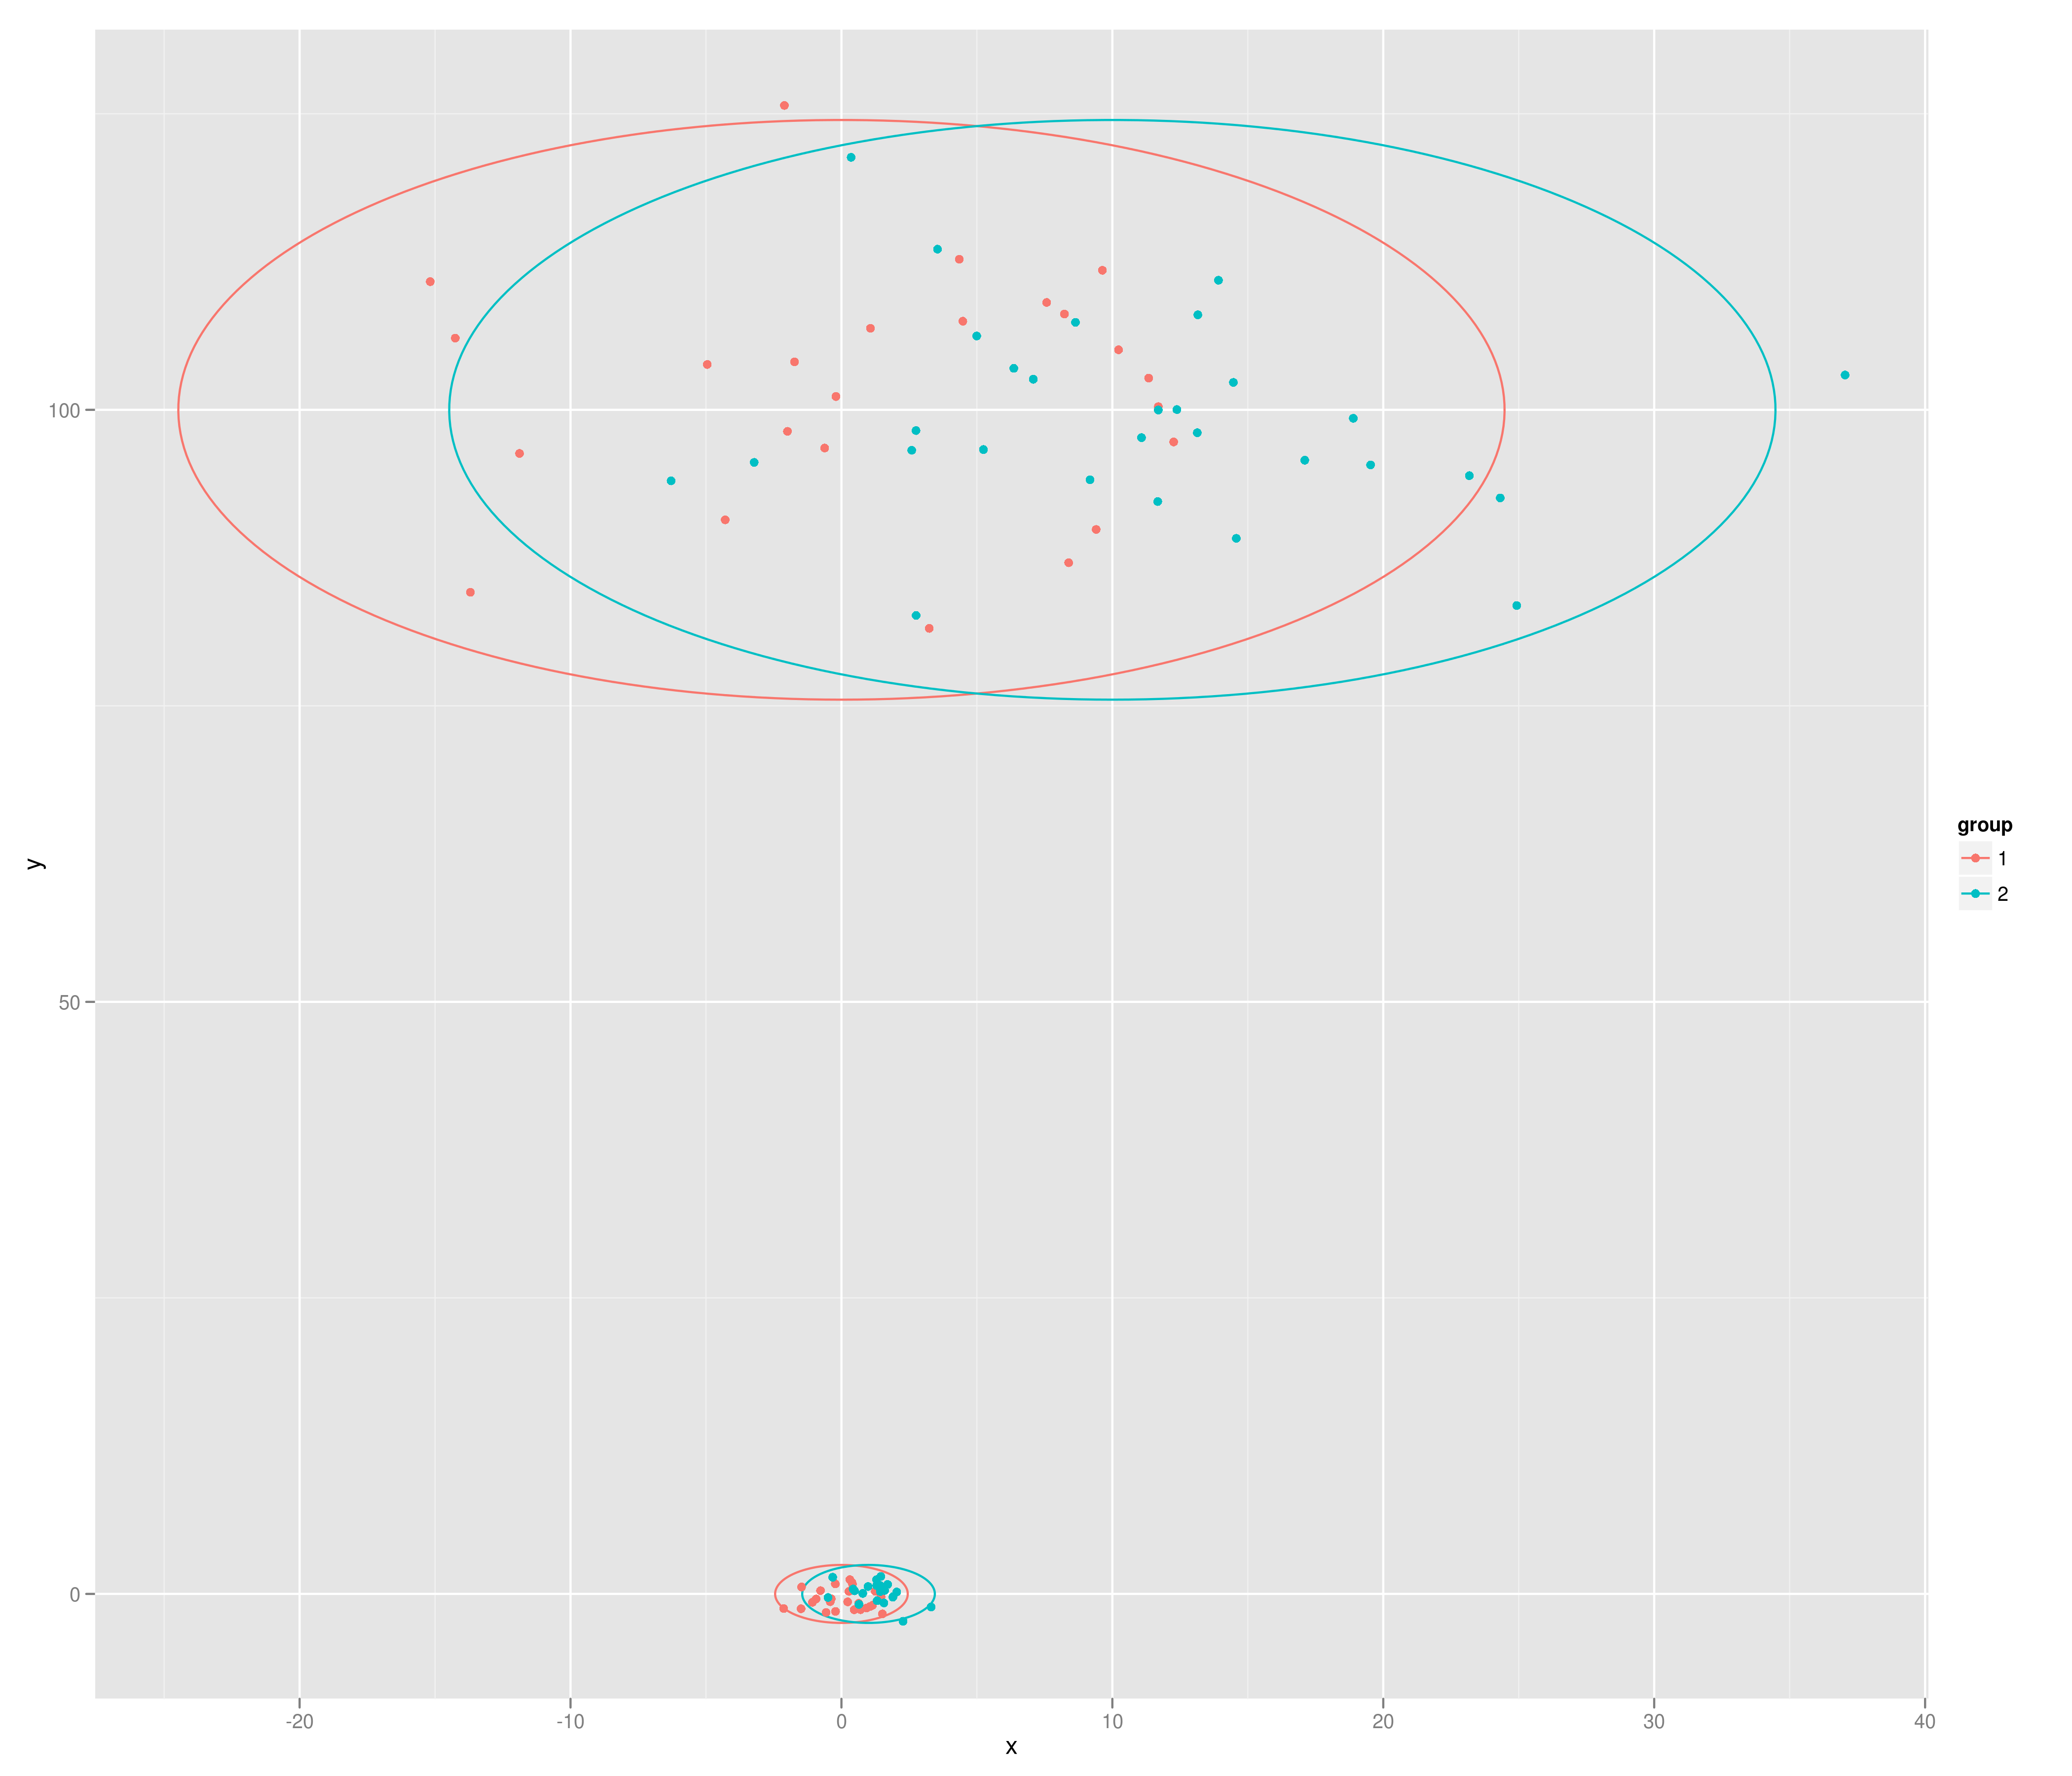
\includegraphics[scale=.3]{vectorial_distributions.png}  
\end{figure}

Here we plot the average power and bootstrap 95\% confidence intervals
(100 simulations) for each RBF kernel individually and MKL on all of
them, faceted on the mixture probability.  So for $p = 0$, we have all
the weight on $\mathcal{N}_2(\mu_2, \Sigma_2)$, and for $p = 1$, we
have all the weight on $\mathcal{N}_2(\mu_1, \Sigma_1)$.  Since the
latter is on a smaller scale, we expect the smaller width RBF kernels
to do better.  We take $C = 1$, and the widths to be from the middle
run of the last section:
\begin{figure}[!ht]
  \centering
  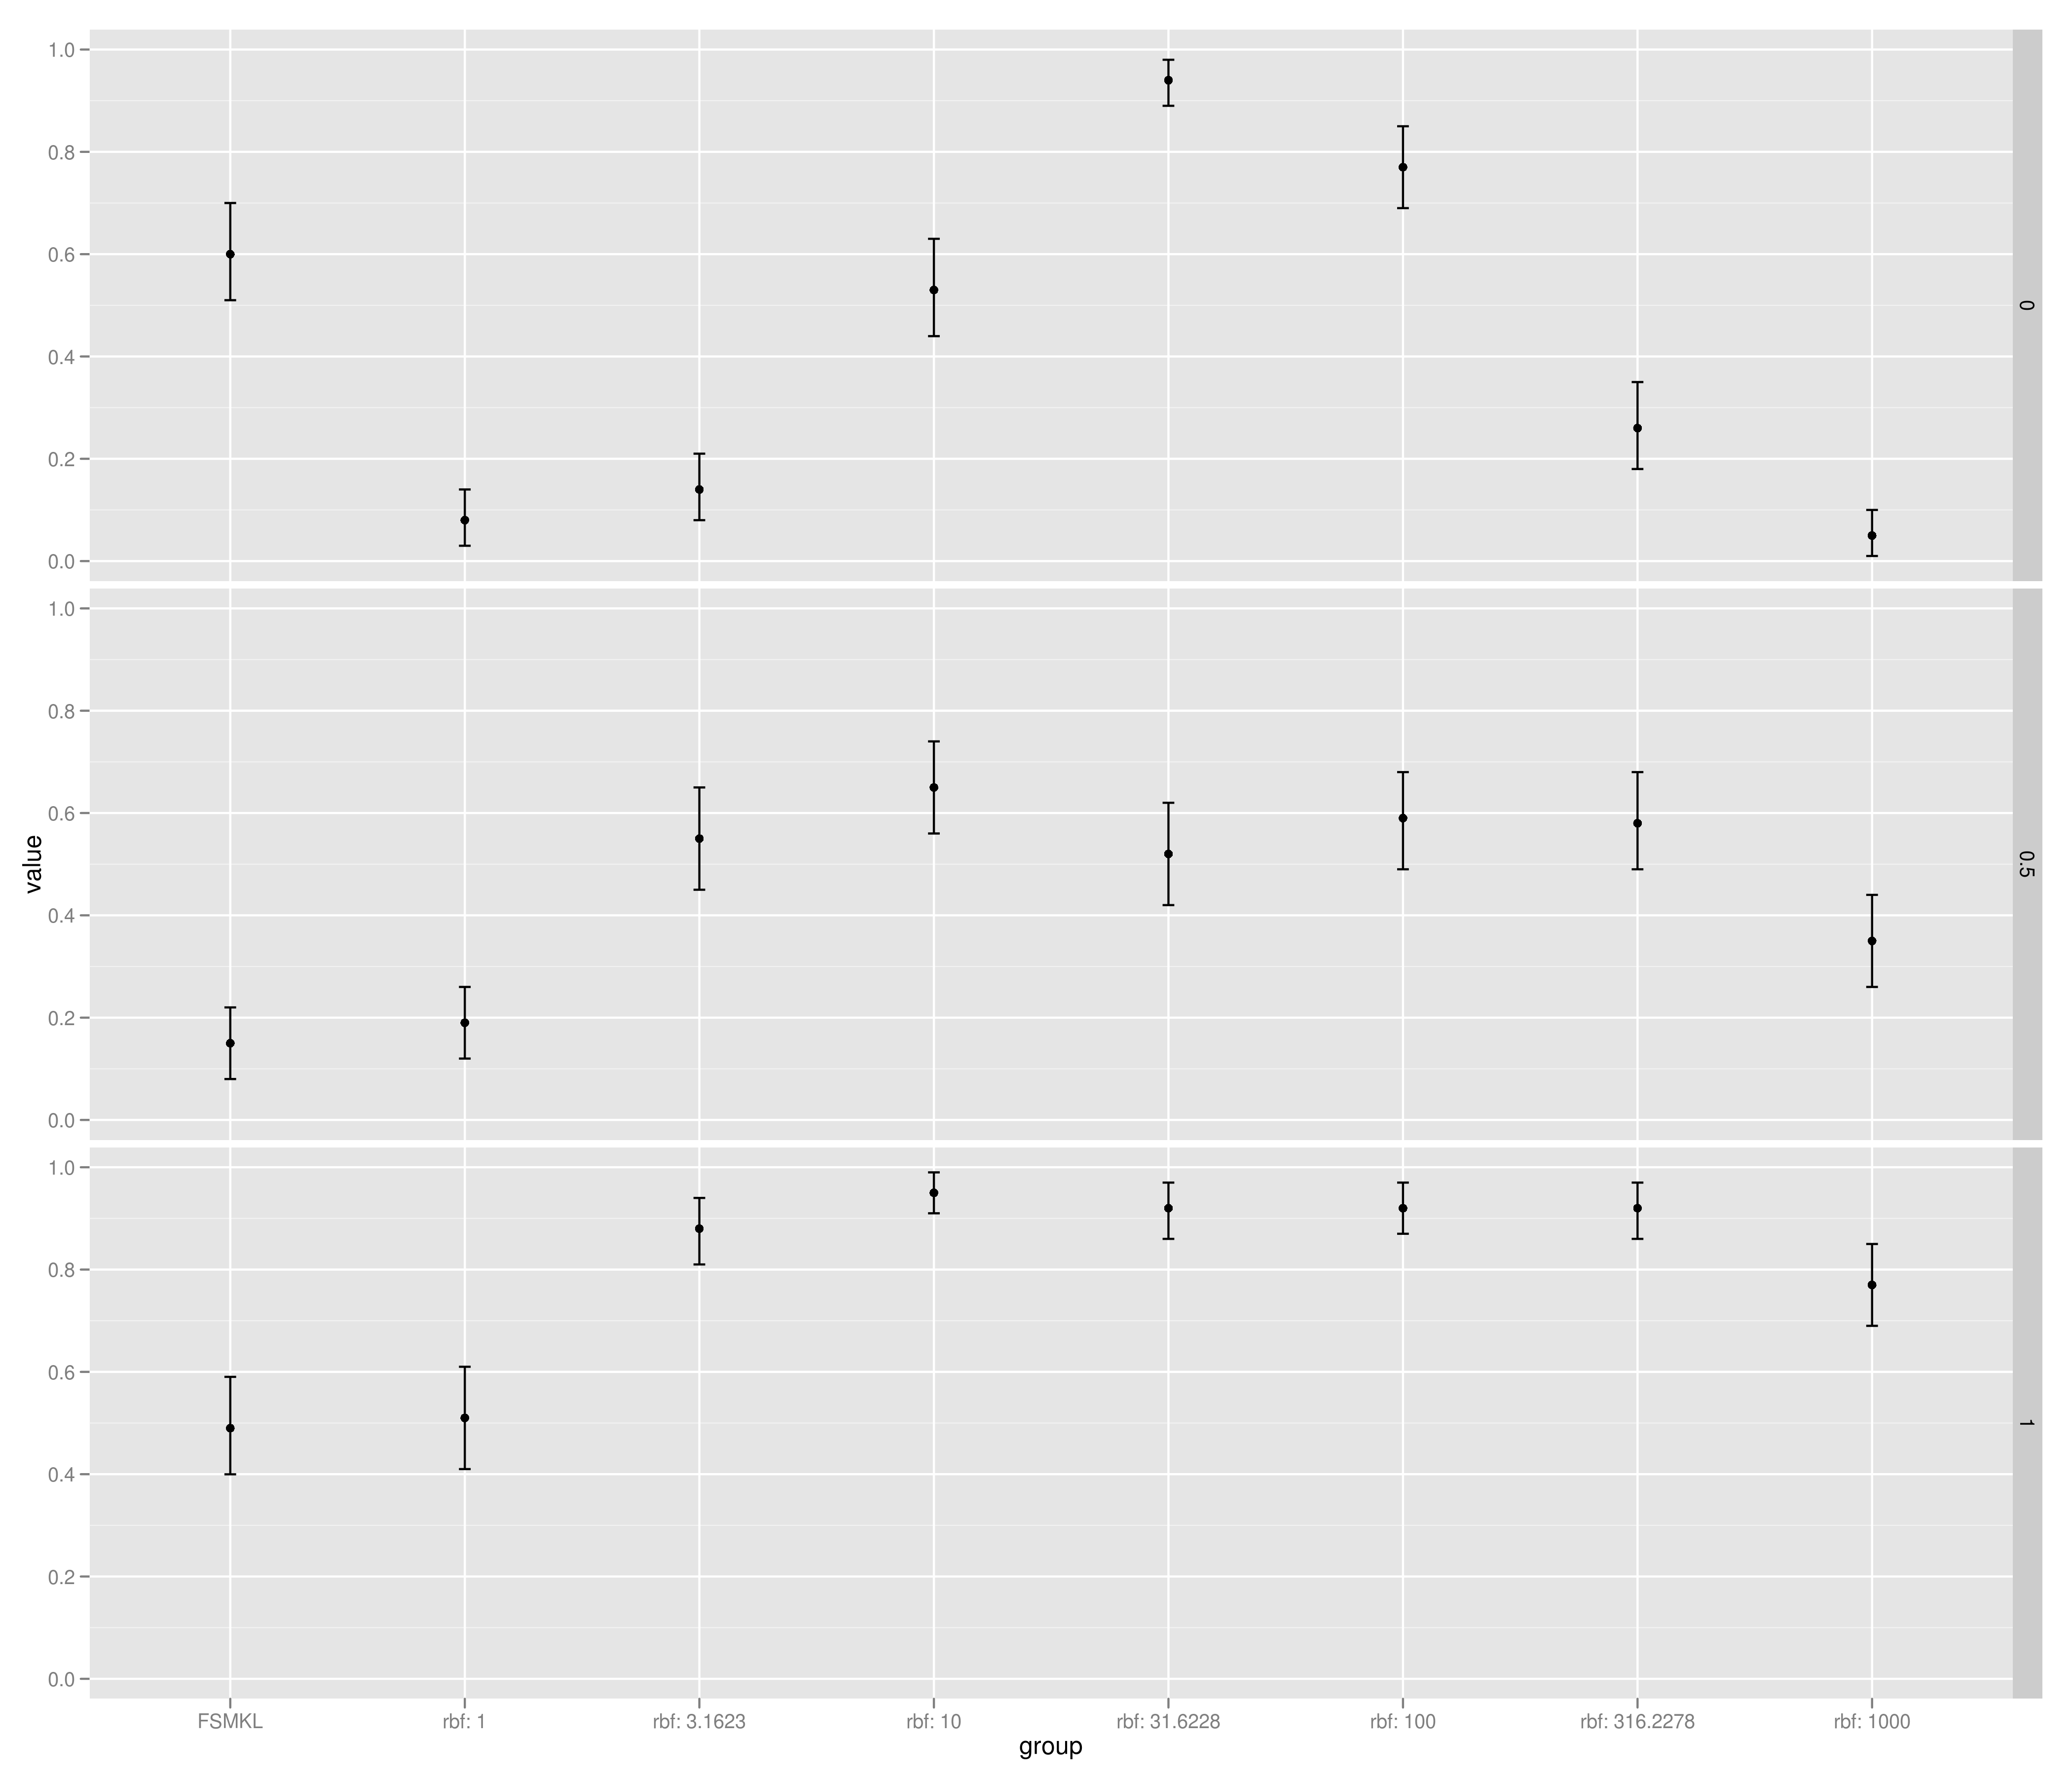
\includegraphics[scale=.3]{vectorial_power.png}
\end{figure}
The smaller distribution ($p=1$) has higher power for smaller kernels,
but the MKL power is about the same as compared with the $p=0$ case.
Both outperform the mixed setting.

Here are the null distributions of the weights and the observed weights:
\begin{figure}[!ht]
  \centering
  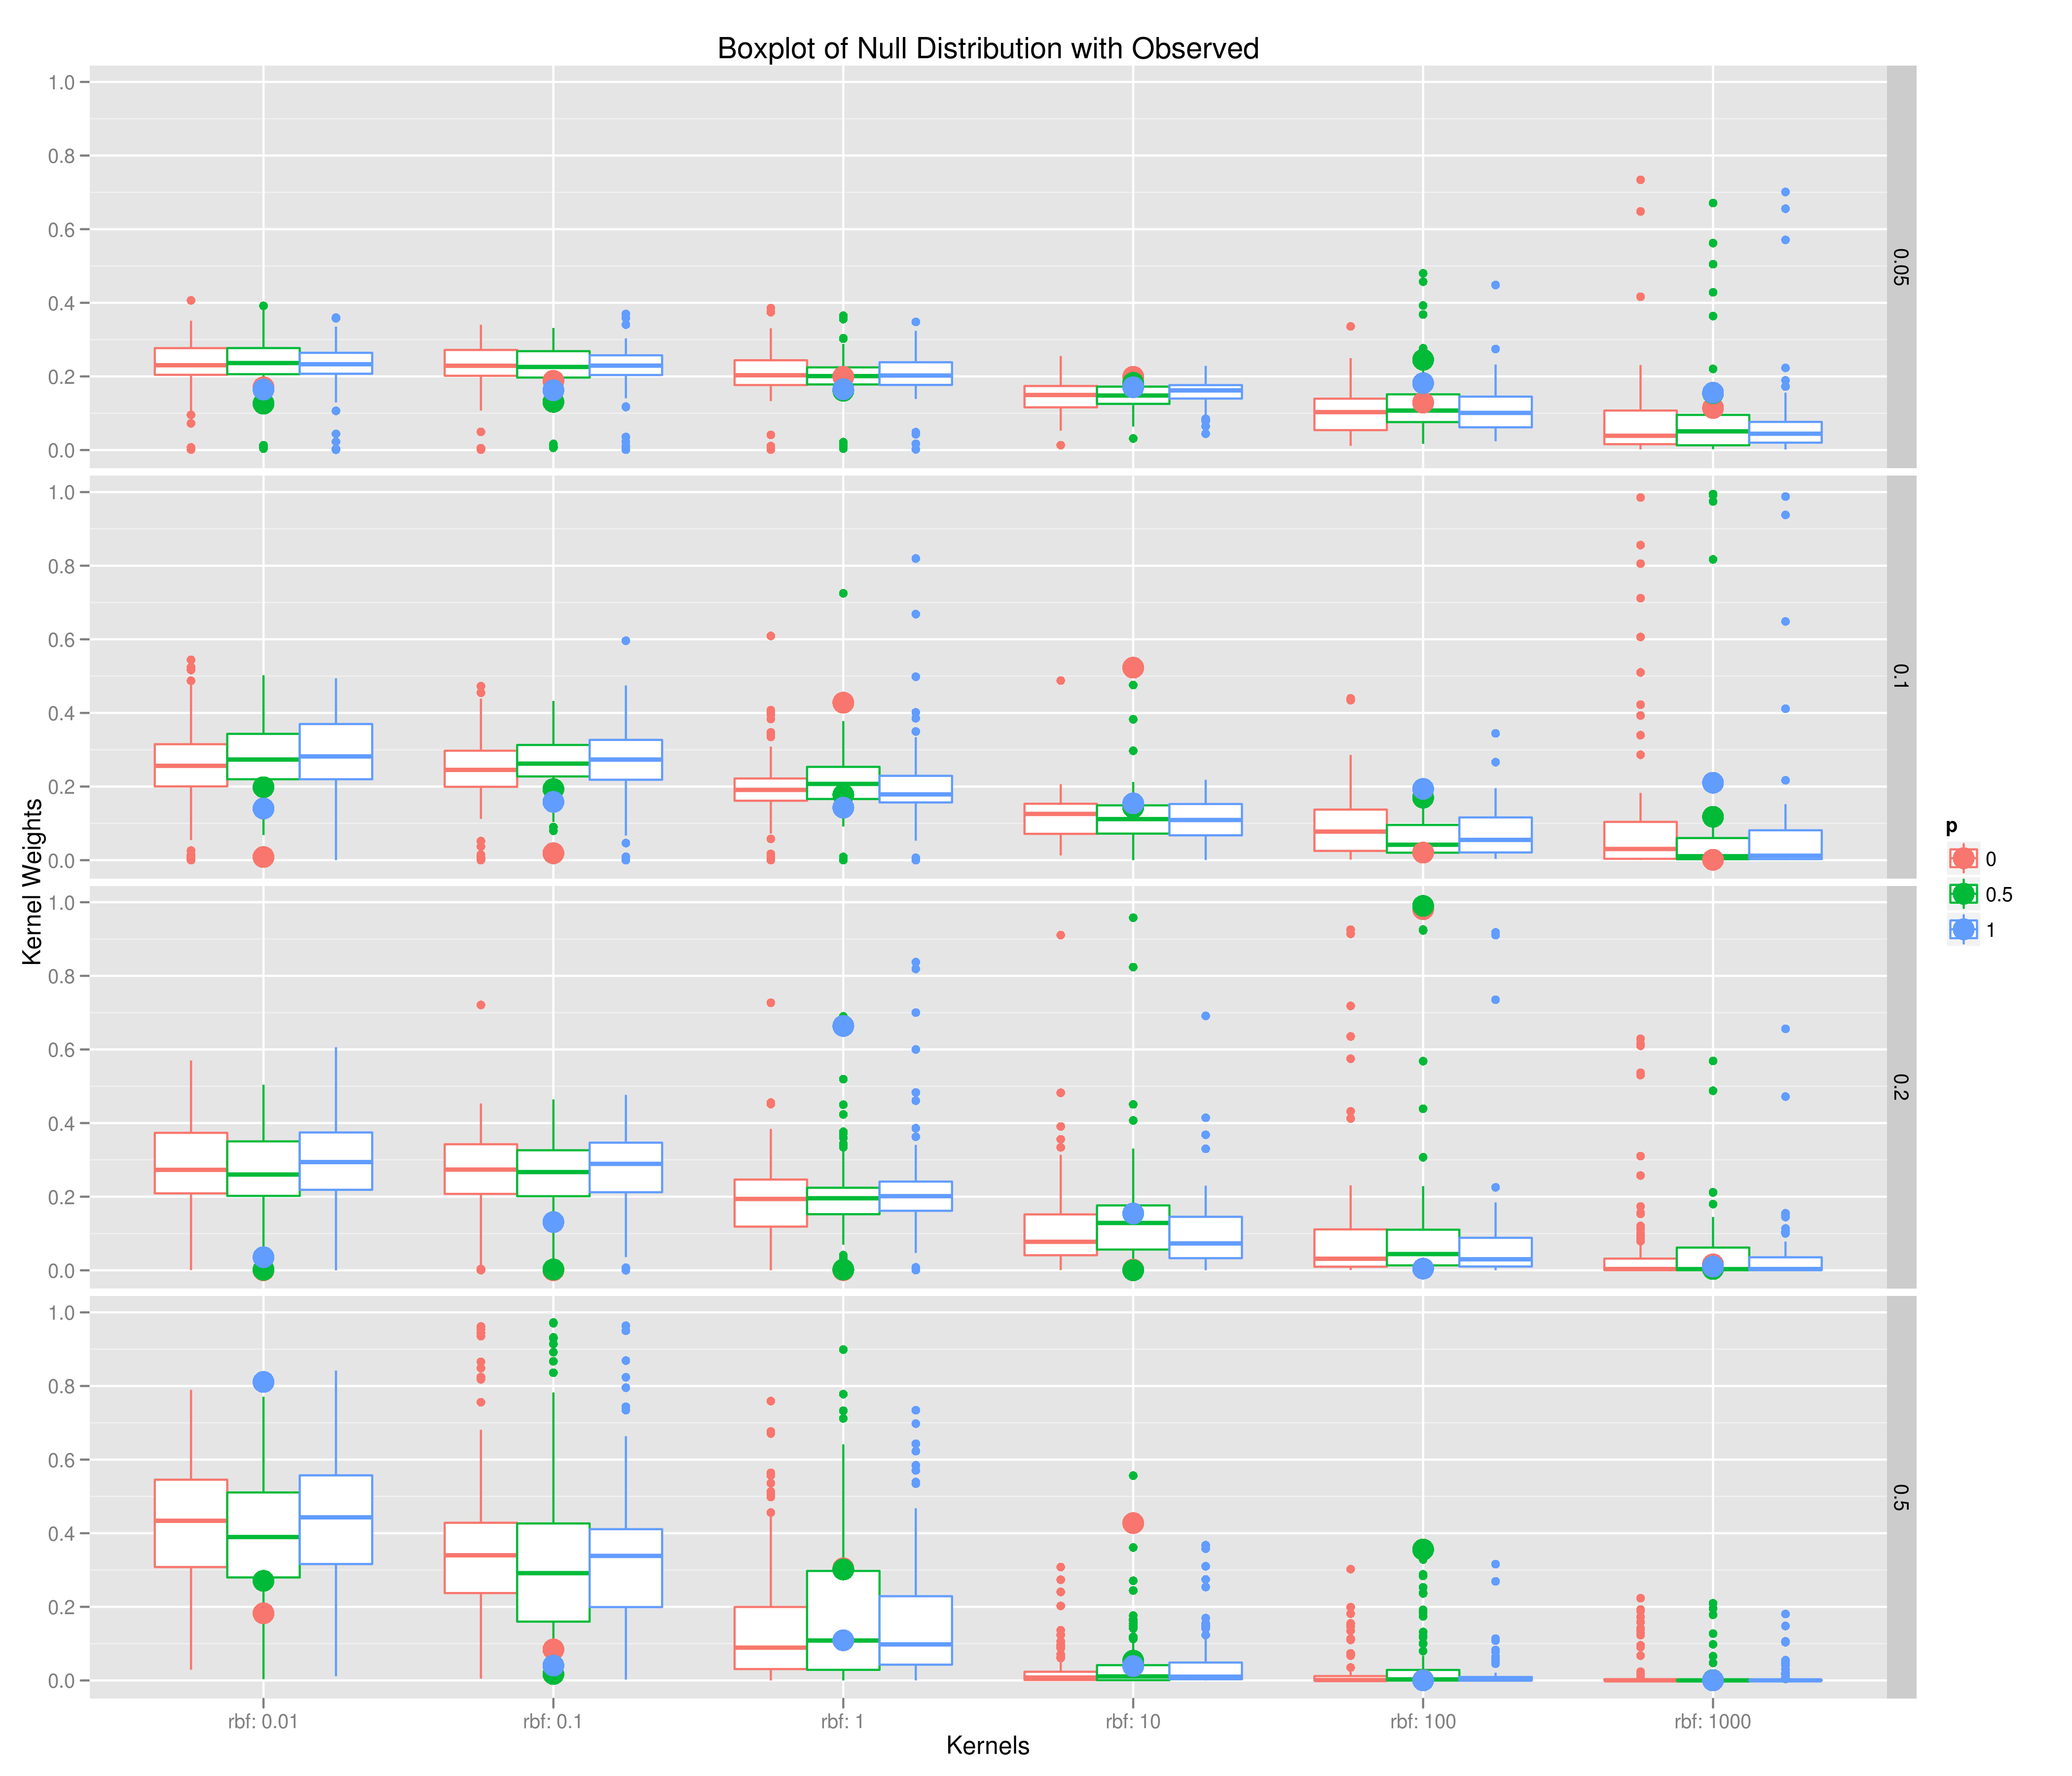
\includegraphics[scale=.3]{vectorial_weights.png}  
\end{figure}

\subsection{Heterogeneous Data}
I created a test
heterogeneous dataset that has two components to it: DNA string and
univariate.  I created the DNA data via a Markov chain because I
wanted the joint distribution of 2-grams to be different from the
product of two 1-grams.  I wanted this dependence so that I could
later pick out differences between two groups with a 2-spectrum kernel
instead of a 1-spectrum kernel.  For the first group, I randomly
picked a starting string according to the stationary distribution and
then proceeded via the transition probabilities.  For the second
group, I had independent draws from the stationary distribution.

The univariate data is simply $\mathcal{N}(\{-\mu, \mu\}, 1)$, and there are 20
samples in each group.  I fixed the kernel training parameter values
and trained a convex combination of 5 kernels on the data via MKL:
Gaussian RBF kernels with parameter .1, .2, .5, and 1, and a
2-spectrum kernel (later I do want to test that the 2-spectrum is
required in this case over the 1-spectrum because of the Markov chain
construction of the data, but I had to add pre-processors and I'm
still not too familiar with shogun yet).

I looked at the kernel weights (so no Friedman test yet) over $\mu = .5,
.6, \ldots, 2.9, 3$.  The weights on, say, the 2-spectrum kernel aren't
monotonically decreasing because of sampling variance: I only ran each
of these once.  I have attached MKL1.png to show that the signal in
the DNA data outweighs (in the sense of yielding a higher MKL weight)
the signal in the univariate part of the data until $\mu = 1.5$ or so.
At that point, the RBF1 kernel takes over.

The pictures from our meeting weren't that compelling, so I've been
looking for better examples.  I decided a reasonable one was the
Christmas star example on page 1548 of
http://eprints.pascal-network.org/archive/00002269/01/sonnenburg06a.pdf

Imagine an outer star (radius 4, 5, 6, 7, 8) with an inner star
(radius 4) inside.  The different stars correspond to different
labelings in the classification problem.  I looked at 5 kernels
individually (RBF with width .01, .1, 1, 10, 1000) and the MKL
combination of all of them).

Here's a heterogeneous data example.  I added string (DNA) data to the
Christmas star example from last week.  So each point is $(l_i, x_i,
y_i, s_i)$ = (label, Christmas star x-coordinate, Christmas star
y-coordinate, DNA sequence).  I generated the DNA by first picking a
random (Poisson) length, sampling the starting point from the
stationary distribution (all 1/4) of the Markov chain, and then
picking according to the transition matrix $M$, where $M_{i,i} = s$ (for
self transition probability) and $M_{i,j} = \frac{(1 - s)}{3}$ for $i \neq j$.

Here are the MKL weights:
\begin{figure}[!ht]
  \centering
    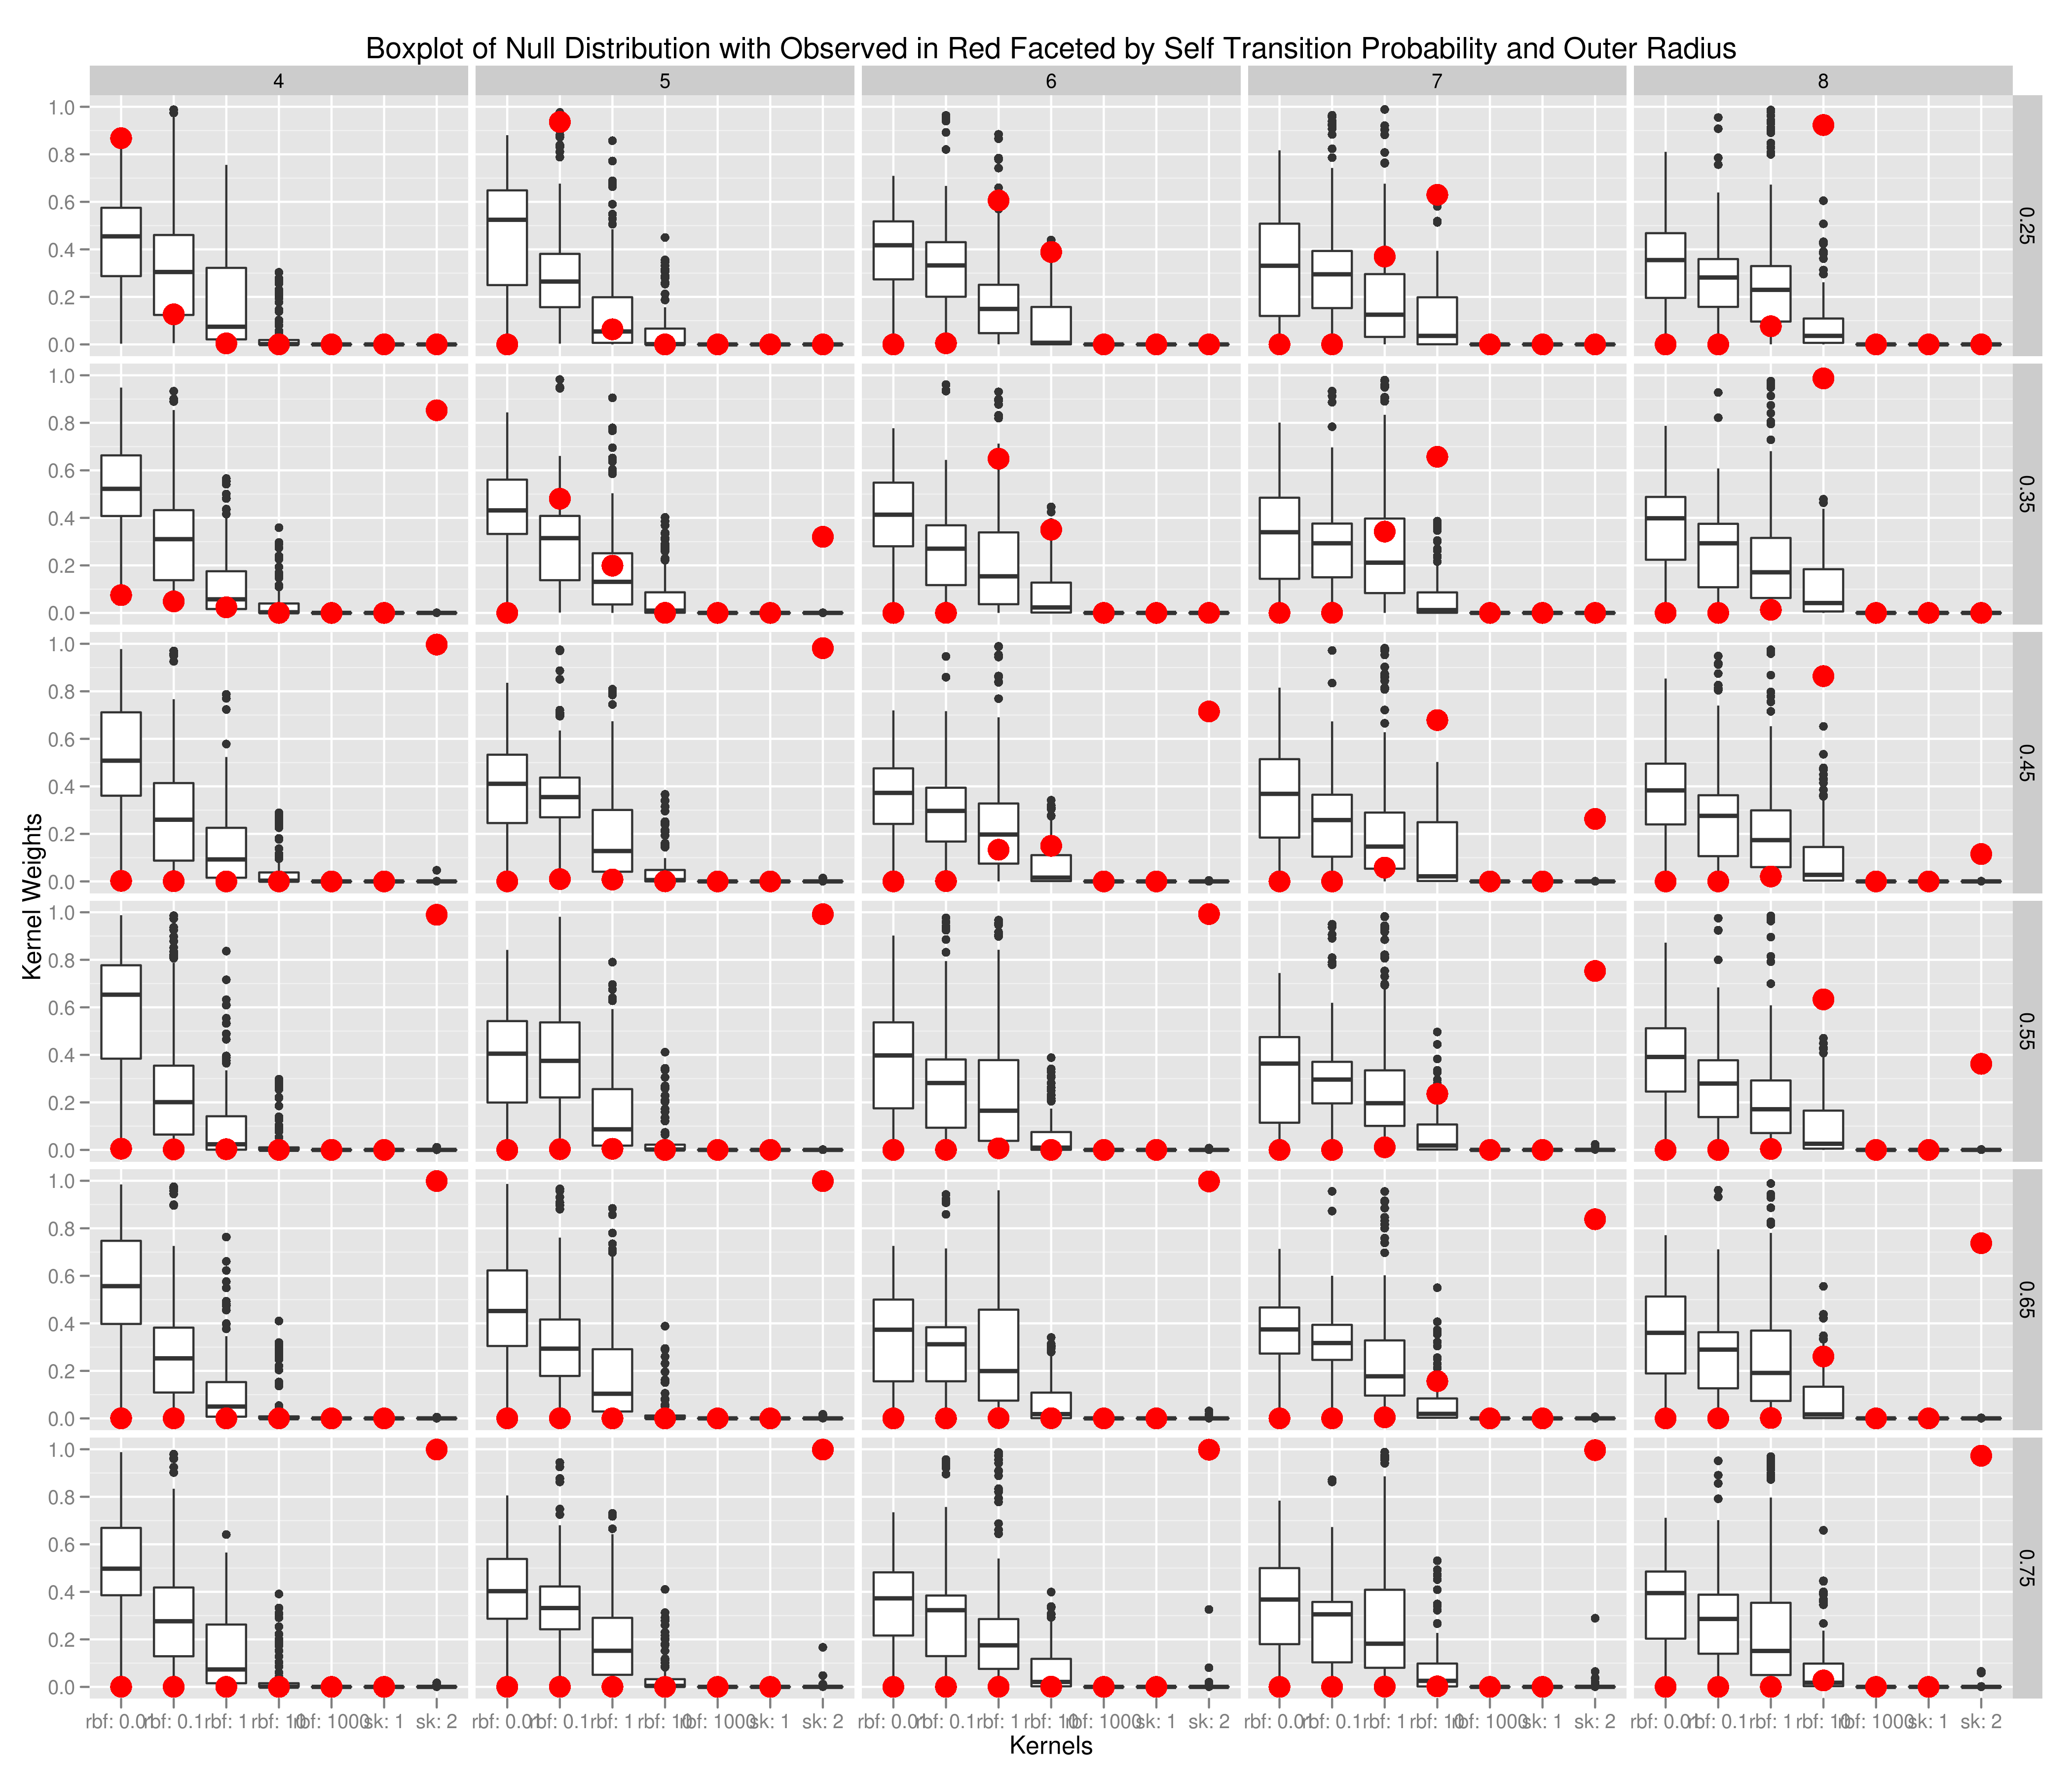
\includegraphics[scale=.3]{mkl_weight_boxplot_christmas_star_DNA.png}  
\end{figure}

And the power:
\begin{figure}[!ht]
  \centering
    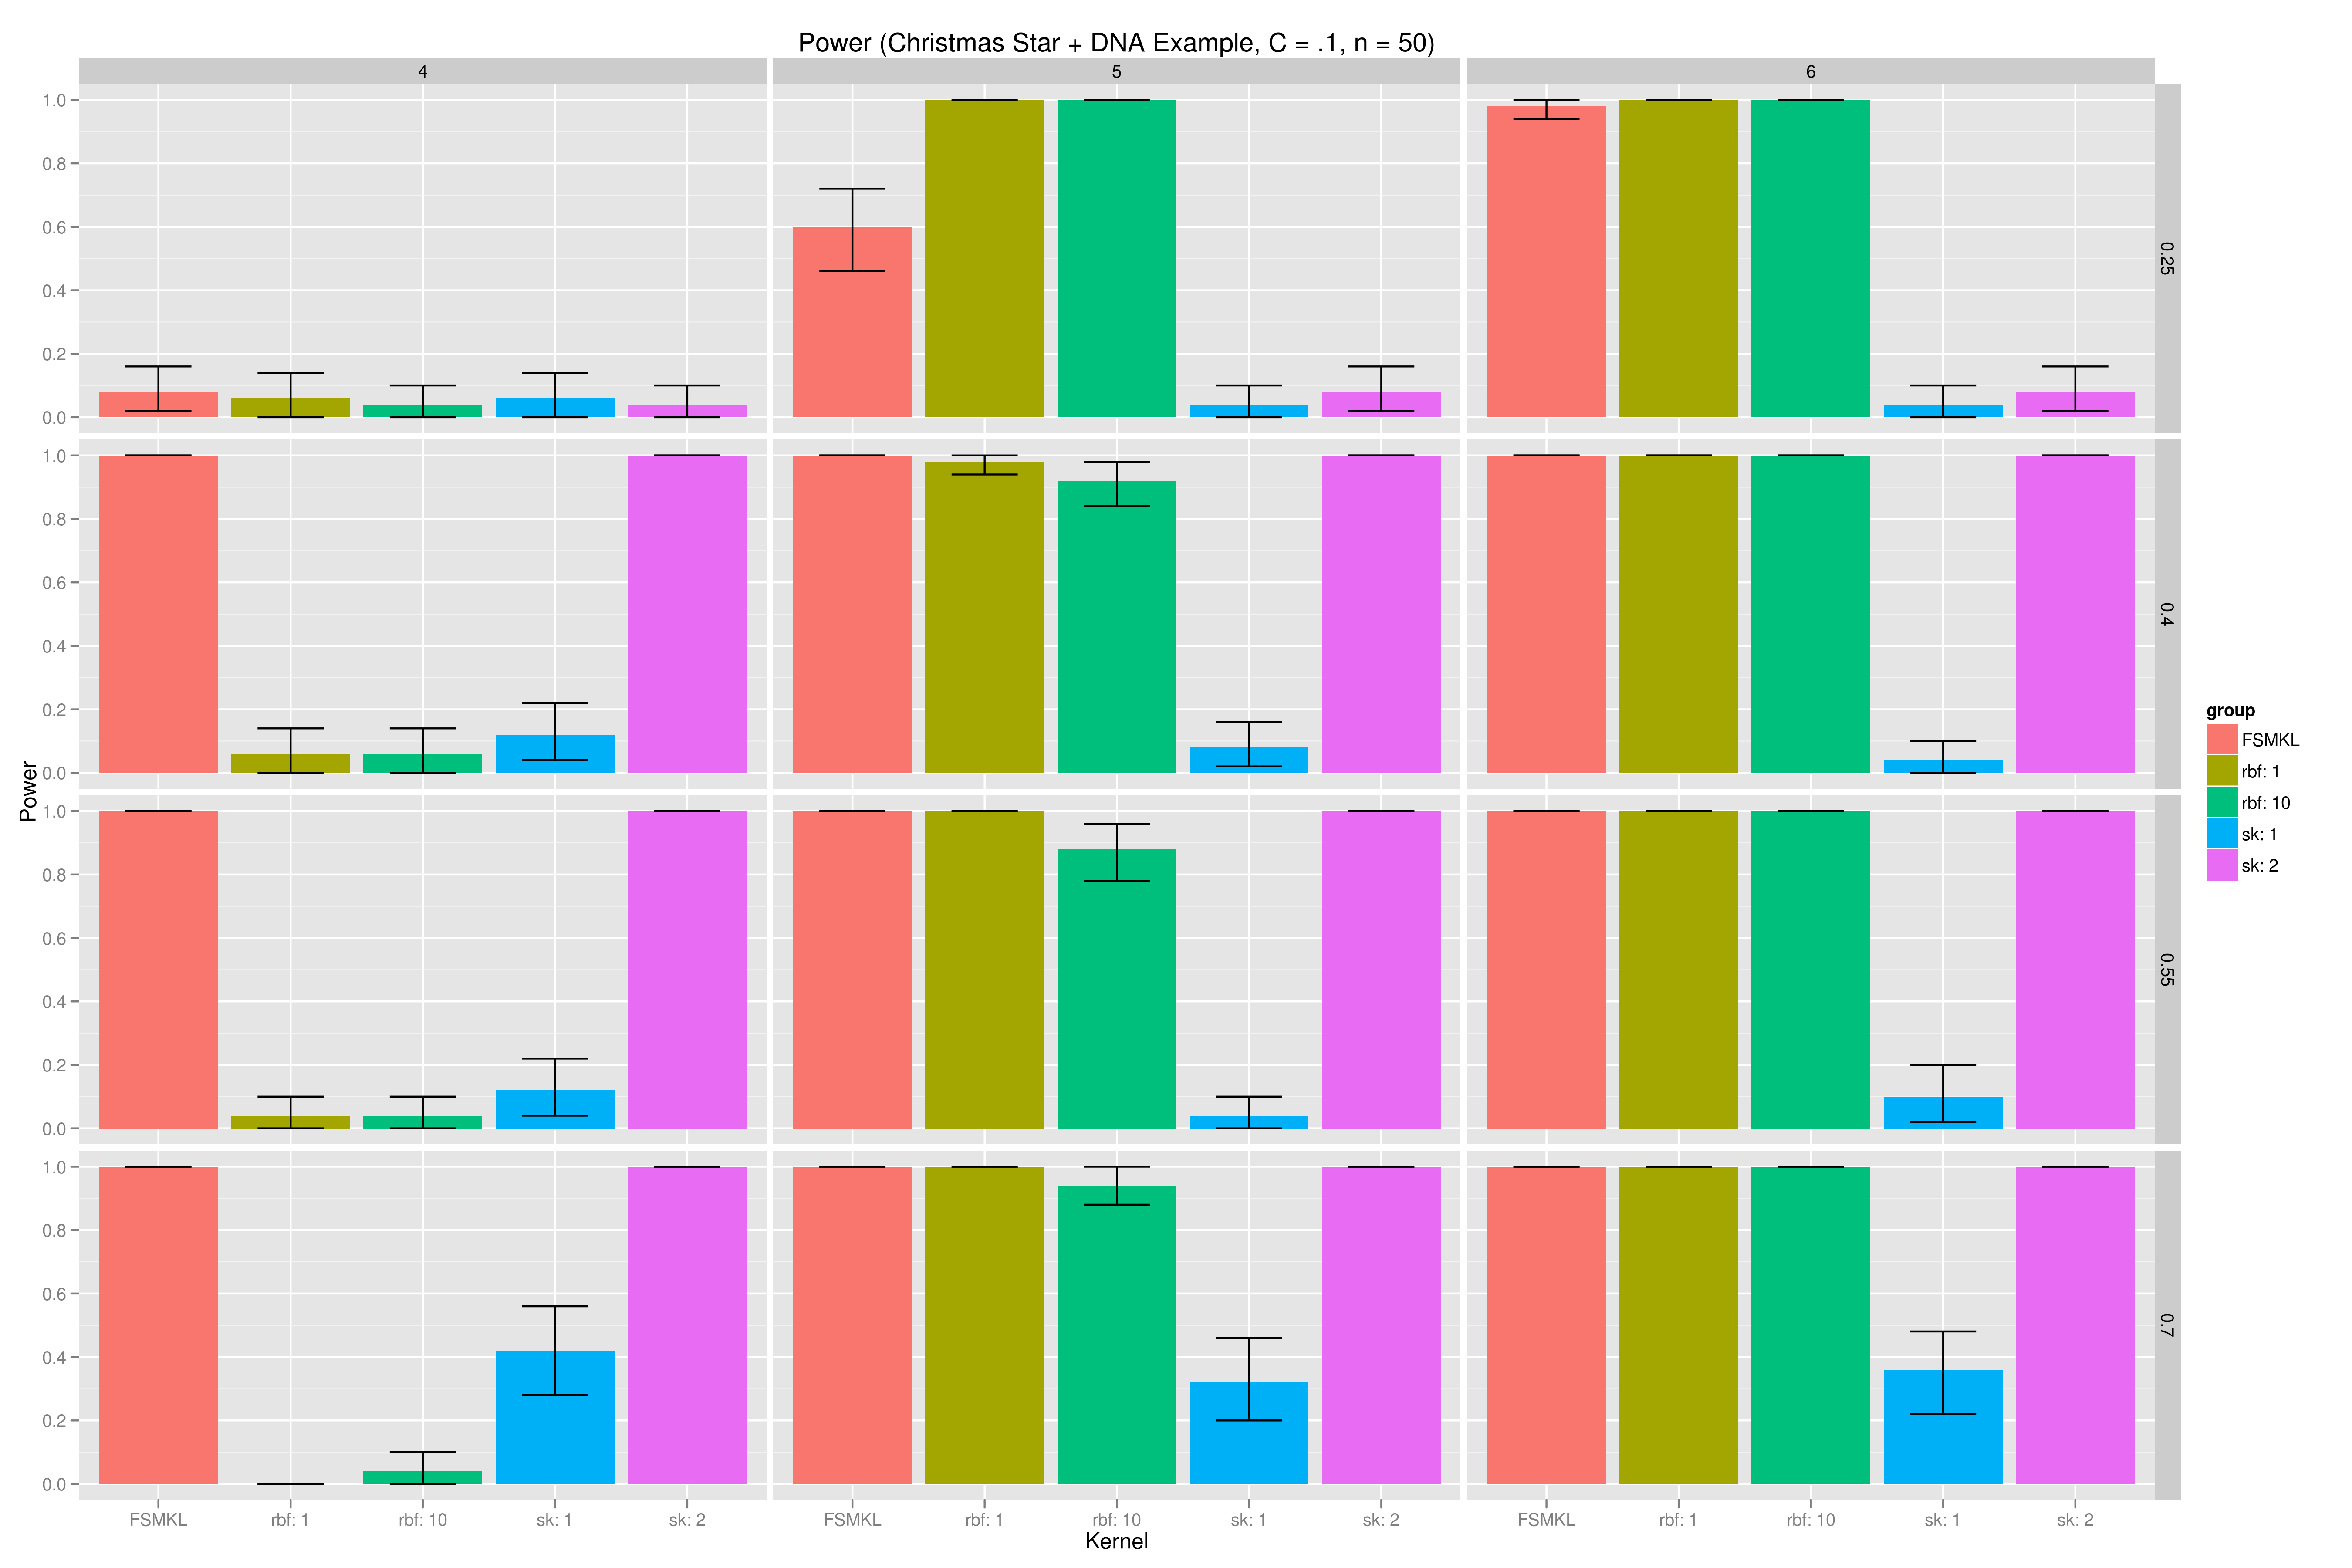
\includegraphics[scale=.3]{power_christmas_star_DNA_facet4.png}  
\end{figure}

The effect of $C$:
\begin{figure}[!ht]
  \centering
      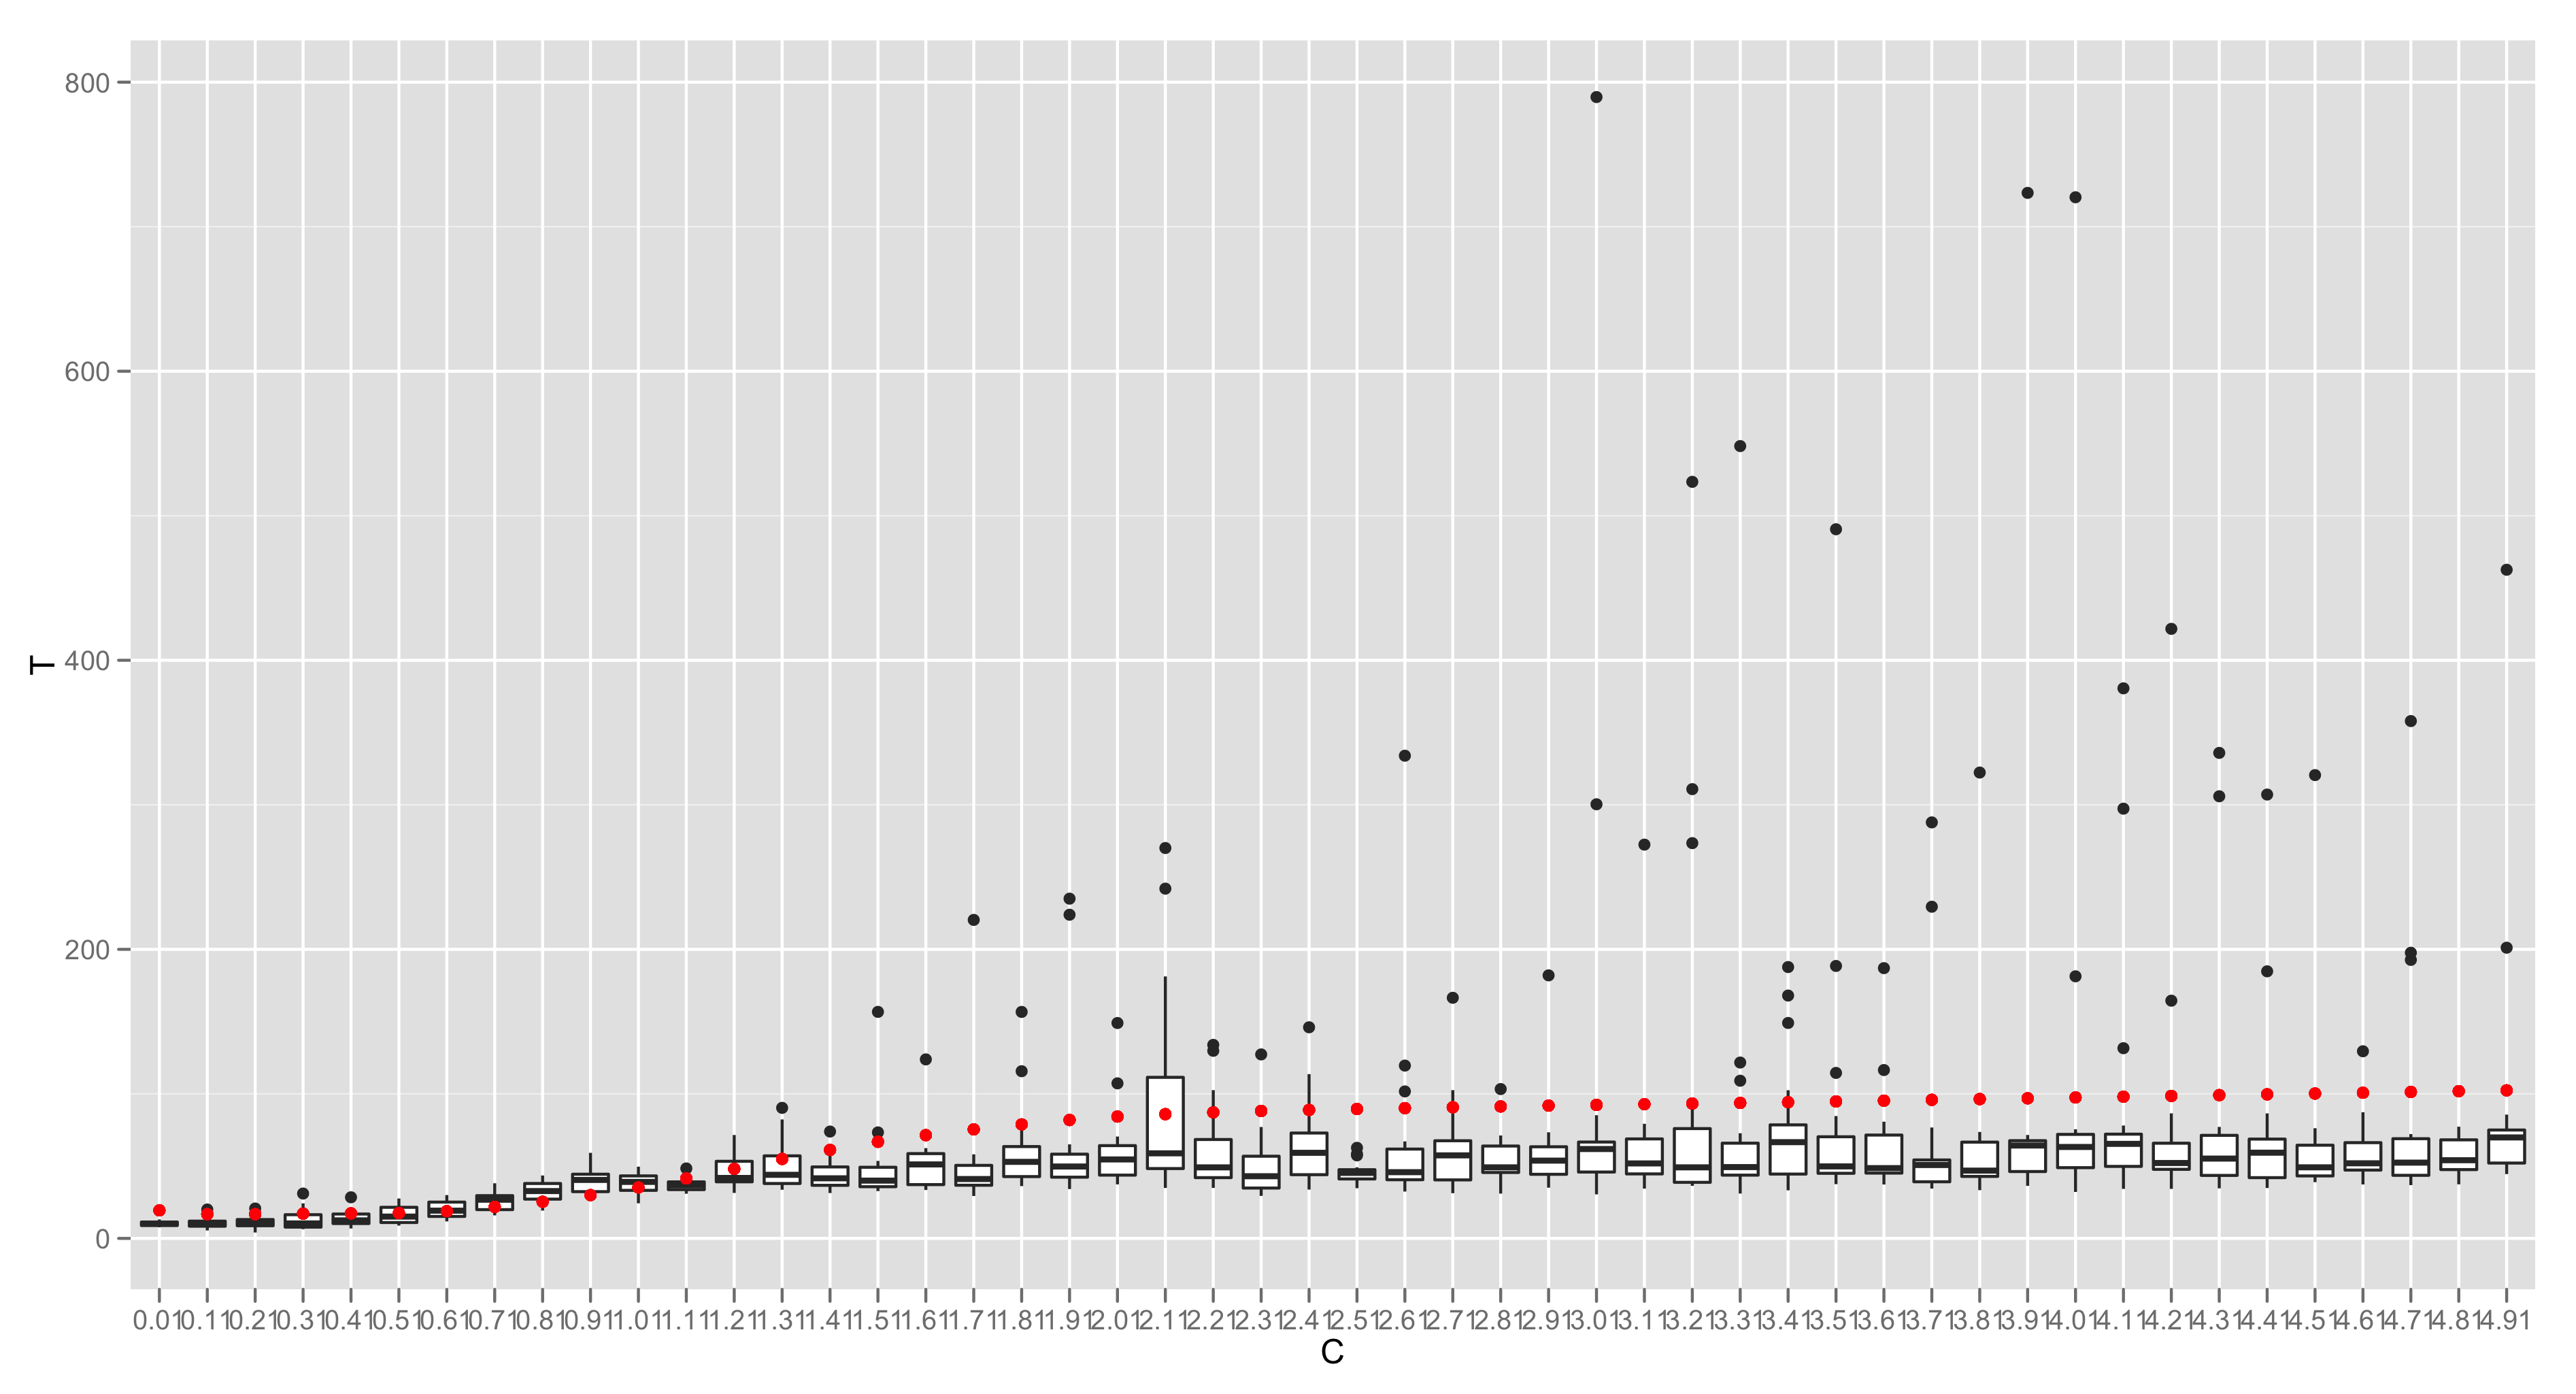
\includegraphics[scale=.1]{tstat_on_c.png}
\end{figure}

$C$ clearly has an effect, especially if you get it very wrong (>.8).
I'm a little disappointed in the performance of MKL but pleased that
it does pick out the right structure in the data.  I'd like to say
that if you know the structure of the data a priori and use that in
the kernel, you will obviously get the best performance.  It seems
like you give up a lot of performance using MKL (maybe too much to
justify its convenience), only doing better than the worst choices of
kernels given.

MKL can pick out the structure of the data:
\begin{figure}[!ht]
  \centering
      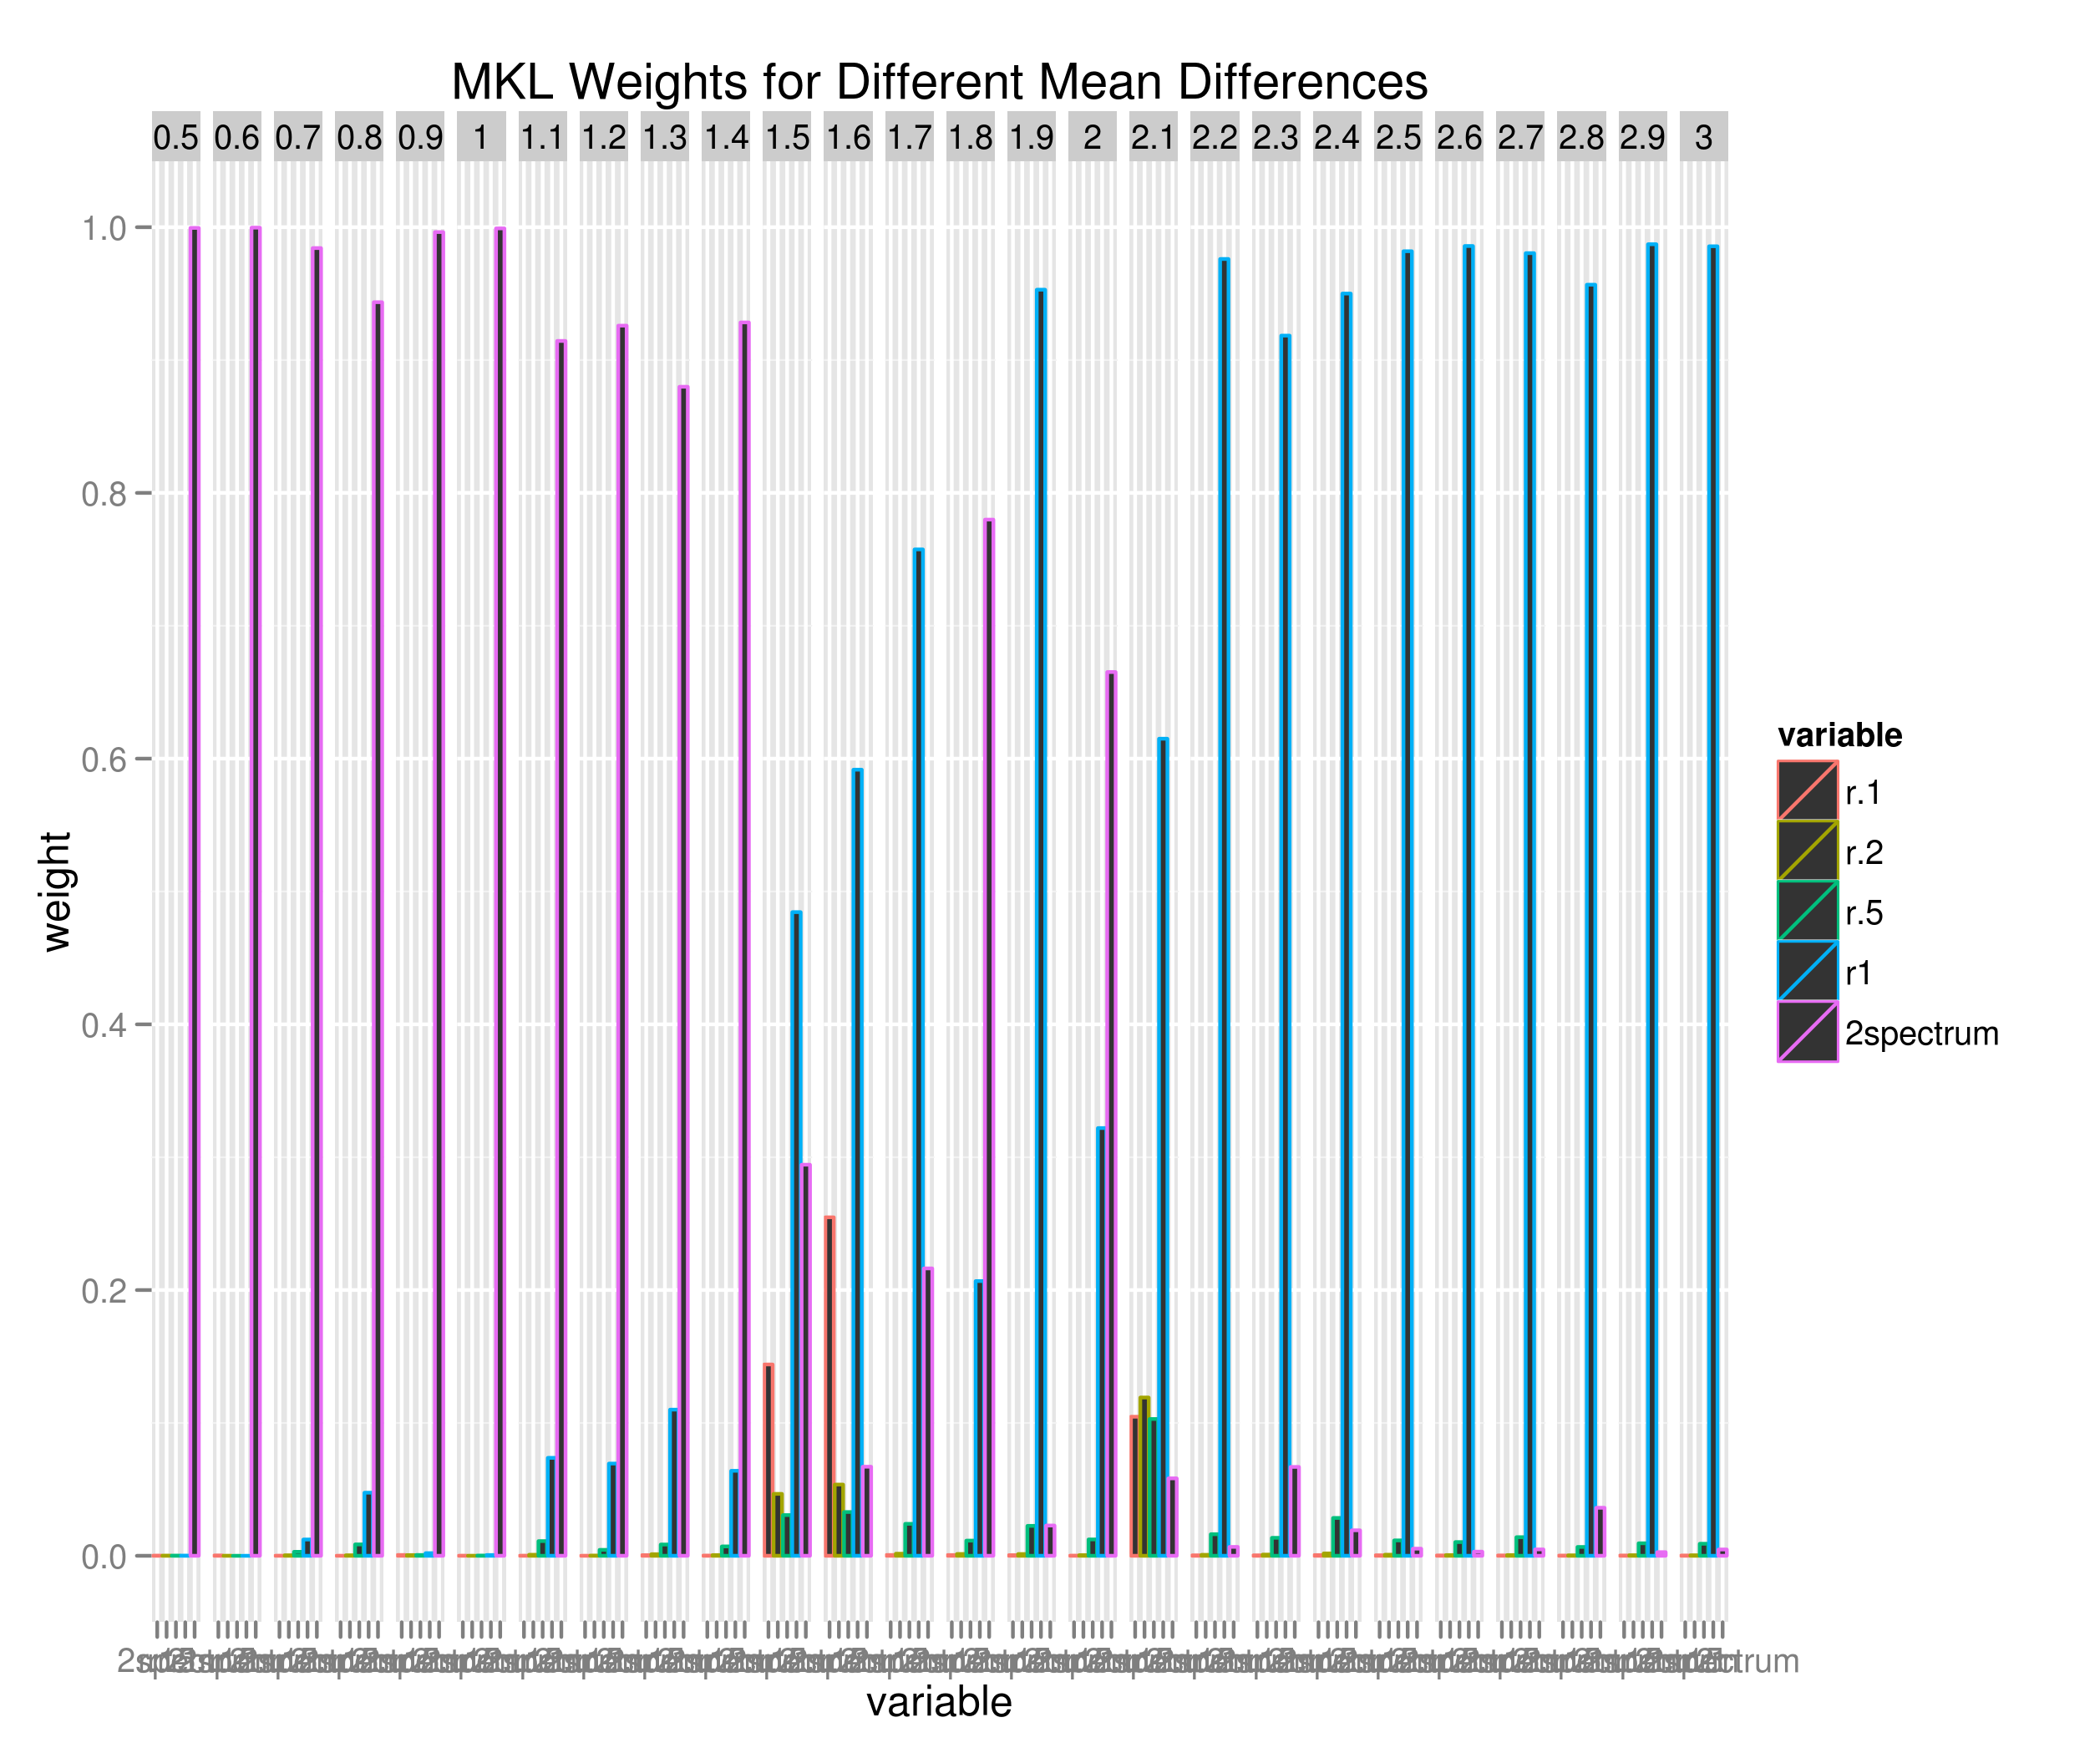
\includegraphics[scale=.5]{MKL1.png}
\end{figure}

\section{Wine Example}
TODO
